\documentclass[10pt,a4paper]{article}
\usepackage[utf8]{inputenc}
\usepackage{amsmath}
\usepackage{amsfonts}
\usepackage{amssymb}
\usepackage{xcolor}
\usepackage{natbib}
\usepackage{graphicx}
%\usepackage[left=1cm,right=1cm,top=1cm,bottom=1.5cm]{geometry}
\usepackage{geometry}
\author{L\'eo Guignard}
\title{Array alignment and interpolation}

\DeclareMathOperator*{\argmax}{arg\,max}
\DeclareMathOperator*{\argmin}{arg\,min}

\begin{document}
\maketitle
\paragraph{}When doing spatial single-cell transcriptomics, beads are recorded from arrays.
Beads are placed on a 2D matrix where each bead is spaced by a given distance $x_{res}$ (resp.
$y_{res}$) along the $x$ (resp.
$y$) dimension (in our case $x_{res}=y_{res}=6 \mu m$).
These distances define the $xy$ resolution (or lateral resolution) of the slice or array.
Then, consecutive arrays are spaced by a given distance $z_{res}$ defining the $z$ resolution (or axial resolution) of the dataset (in our case $z_{res}=30\mu m$).
\paragraph{}Because the arrays are physically moved between their slicing and their acquisition, they are not acquired within the same frame (meaning that they are not aligned).
In order to reconstruct a 3D representation of the single cell transcriptomics of the acquired embryo and to do full 3D spatial analysis, it is necessary to align consecutive arrays to recover the spatial integrity of the specimen.
Moreover, because the axial resolution is significantly greater than the lateral one, in some cases, it is necessary to interpolate the data between the arrays.
\paragraph{}In the following section we will describe how this alignment was performed together with how the beads were interpolated between arrays.
\section{Notation}
\paragraph{}We define our dataset as a set of arrays \(\mathcal{P}=\{P_i\}\).
The function $c_P$ maps a array to its height coordinate $z_i$: \(c_P: P_i\in \mathcal{P} \rightarrow z_i \in \mathbb{R}\).
Each array $P_i$ is itself a set of beads, \(P_i=\{b_{ij}\}\) and similarly to the arrays, the function \(c_b\) maps a bead \(b_{ij}\) to its \(xy\) coordinate within the array: \(c_b:b_{ij}\in P_i\rightarrow (x,y)\in \mathbb{R}^2\).
From \(c_P\) and \(c_b\) we define the function \(c:b_{ij}\in P_i\rightarrow (x,y,z)\in\mathbb{R}\) which maps a bead to its 3D spatial coordinate.
Note that \(c_P\) defines a total order on the arrays.
Let then \(\mathcal{P}\) be ordered such that \(\forall i,j,~P_i<P_j\iff c_P(P_i)<c_P(P_j)\).
%%
\paragraph{}Moreover, using the previously described analysis, we can associate each bead to the tissue it most likely belongs to, the function \(T:b_{ij}\in P_i\rightarrow t\in\mathcal{T}\) where \(t\in\mathcal{T}\) maps each bead to a unique identifier for the tissue it belongs to. \(\mathcal{T}\) is the set of possible tissues previously identified.
Similarly, to each bead is associated a value for each given gene analysed in the dataset.
This value is correlated to the level of expression of said gene for said bead.
Given a gene \(g\), we define the function \(E_g:b_{ij}\in P_i\rightarrow e\in\mathbb{R}\) which maps the value \(e\) of expression of the gene \(g\) to the bead \(b_{ij}\).
%%
\section{Pre-processing}
\subsection{Removing the remaining outliers}
\paragraph{}Before aligning the arrays it is possible to remove beads that are likely to be noise.
Within a given tissue, noisy beads were detected as the beads that were spatially further away from their neighbors than the normal distribution of the spatial distances between beads.
To assess the normal distribution of spatial distances between beads of a given tissue, we first computed the distance between any given bead and its closest bead from the same tissue type.
We then analysed the distribution of these distances by fitting a gaussian mixture model, with a number of components equal to \(n_{components}\) (in our case we used \(n_{components}=3\).
When using 3 components, the \(1^{st}\) and \(2^{nd}\) components are assumed to be real.
The \(3^{rd}\) component, with the higher mean, is the distribution of distances of noisy beads.
We then discarded all the beads that had a distance to their closest neighbor from the same tissue which had a probability to belong to the first or second component were lower than \(th_{gmm}\) (in our case we used \(th_{gmm}=0.6\%\)).
This pre-processing step is not mandatory but it can help getting more accurate results. The value might vary depending on the sample and tissue analyzed.
\section{Aligning the arrays}
\paragraph{}As previously mentioned, due to the nature of the acquisition process, consecutive arrays do not live within the same frame.
They are therefore not spatially comparable.
\paragraph{}To align the arrays and register them onto the same frame, we first chose our first array in \(\mathcal{P}\), \(P_0\), as the reference array.
We then registered each following slide to its preceding one: \(P_1\) is registered onto \(P_0\), \(P_{i+1}\) is registered onto \(P_{i}\) and so on and so forth.
Ultimately we can compose all the transformations together to register any array onto the first array.
To compute the transformation necessary to register two consecutive arrays, we first performed a coarse grain alignment using the center of mass of a subset of the different tissue types.
We then refined the alignment by pairing beads across the arrays and by aligning them.
\subsection{Coarse grain alignment}
\paragraph{}We first chose a subset of tissues \(\mathcal{L}\subset\mathcal{T}\) that are spatially localised (for example heart tube precursor beads or somite precursor beads).
We then discarded (only for the coarse grain alignment) tissues that were spread in space (for example blood precursor beads).
An exhaustive list of the discarded tissue types can be found below.
\paragraph{}Then we computed the alignment transformation (\(r_{i\leftarrow j}^*\), registering the array \(P_j\) onto the array \(P_i\)) as the rigid transformation (translation plus rotation) that minimizes the sum of the squared distances between corresponding tissue types center of mass:
\begin{eqnarray}\label{eq:rigid}
r_{i\leftarrow j}^*&=&\argmax_{r\in\mathcal{R}} \big\{\sum_{t\in \mathcal{L}}||COM_i(t)-r[COM_j(t)]||_2\big\}
\end{eqnarray}
where \(COM_i(t)\) is the position of the center of mass of the tissue \(t\) in the array \(i\), \(||\cdot||_2\) is the L2 norm and \(\mathcal{R}\) is the set of all rigid transformations.
\(r[COM_j(t)]\) is therefore the position of the center of mass of the tissue \(t\) in the array \(j\) after application of the rigid transformation \(r\).
\paragraph{}We then applied the composition of the necessary transformations to register all arrays onto the first array.
For example, to register the array \(j\) onto the array \(0\), we applied the transformation \(r_{0\leftarrow j}^*=r_{0\leftarrow 1}^*\circ r_{1\leftarrow 2}^*\circ \cdots \circ r_{j-1\leftarrow j}^*\).
\subsection{Alignment refinement}\label{subsec:ali-ref}
\paragraph{}To refine the alignment, we then paired beads from consecutive arrays.
Only beads from the same tissue types could be paired.
The pairing was the one that minimizes the sum of the distances between paired beads (using the solution of the linear sum assignment optimization).
The distances were computed after applying the coarse grain transformation.
From this pairing, as previously, we computed the rigid transformation \(R^*_{i\leftarrow j}\) that minimizes the sum of the squares of the distances between the paired beads (see eq.\eqref{eq:rigid}).
\section{In between array interpolation}
\paragraph{}As shown earlier, the distance between two consecutive beads within the same array is significantly smaller than the one between two arrays (one order of magnitude in our case, 6\(\mu m\) versus 30\(\mu m\)). This property makes it that some analysis of the 3D volume of the embryo is difficult or even not possible. If one wants to study a plane that is tilted by a small angle to the original array planes, the beads become too scarce. To overcome this issue, we designed an algorithm to interpolate beads in between arrays. The goal is to create beads where there would likely be and to assign to these interpolated beads gene expression values that are the most likely values.
\paragraph{}To interpolate beads between arrays, we first paired beads belonging to the same tissues (similarly to the pairing that was done in \ref{subsec:ali-ref}) to construct paths of beads (see Fig. \ref{fig:interp} A-B). We then assume a smooth continuity of gene expression and position to compute the interpolation. This smooth and continuous hypothesis on the system is the basis of the interpolation. It is important to keep this hypothesis in mind when doing any further analysis since it might not apply to all samples or tissue types.
\subsection{Bead pairings and paths}
\paragraph{}The first step towards in-between array interpolation is to build a path of beads from consecutive arrays.
These paths were built by pairing beads from consecutive arrays.
Beads were paired based on their spatial proximity.
As previously, we used a linear assignment algorithm to pair beads.
Linear sum alignment requires that a positive cost is computed between any beads that can be paired together.
Here, we used as our cost function the Euclidean distance (hence the spatial proximity bead pairing).
The bead pairing between consecutive arrays creates paths of beads. A path of beads is a series of beads that are paired sequentially by the array to array pairing.
For example \(b_{i,j}\) is paired to \(b_{i+1,k}\) which is paired to \(b_{i+2,l}\). These paired beads then create the path \(Pa_{i,j}=(b_{i,j}, b_{i+1,k},b_{i+2,l})\).
\paragraph{}Because each path does not start (resp. end) at the first (reps. last) array of the sample, to avoid abrupt and artificial stops of the paths, we computed intermediate beads which would mark the most likely end of the path (see Fig. \ref{fig:interp} C). The position of these beads added in between arrays (let them be \(b^{proj}_{i,j}\)) was computed as follow:
\begin{equation}\label{eq:proj}
c(b^{proj}_{i,j})=c({b_{i,j}})+\frac{n}{|\mathcal{N}^p_{i,j}|}\sum_{b_{i,k}\in \mathcal{N}^p_{i,j}}\overrightarrow{b_{i,k},p(b_{i,k})}
\end{equation}
where \(p(b_{i,k})\) is the projection of \(b_{i,k}\) in the following array. \(\mathcal{N}_{i,j}\) is the set of beads that are neighbors of \(b_{i,j}\) according to the Gabriel graph tessellation of the set of beads for a given array.
\(\mathcal{N} ^p_{i,j}\subset \mathcal{N}_{i,j}\) is the subset of neighbors of the bead \(b_{i,j}\) that have a projection, meaning that \(p(b_{i,j})\) exists.
\(n\) is the fraction of the average projection to consider. \(n\) is computed with regard to the distance of the bead \(b_{i,j}\) to its closest neighbor that has a projection.
The closer a bead is to a bead with a projection, the larger \(n\) will be, meaning that if a bead is close to a bead that is linked to another bead in the following array, the longer it will exist in between the arrays.
Note that the Gabriel graph tessellation is a decimation of the more classical vorono\"i tessellation which avoids most of the usual issues of the vorono\"i tessellation especially when it comes to concave set of positions (see \cite{mcdole:2018}).
\begin{figure}
\center
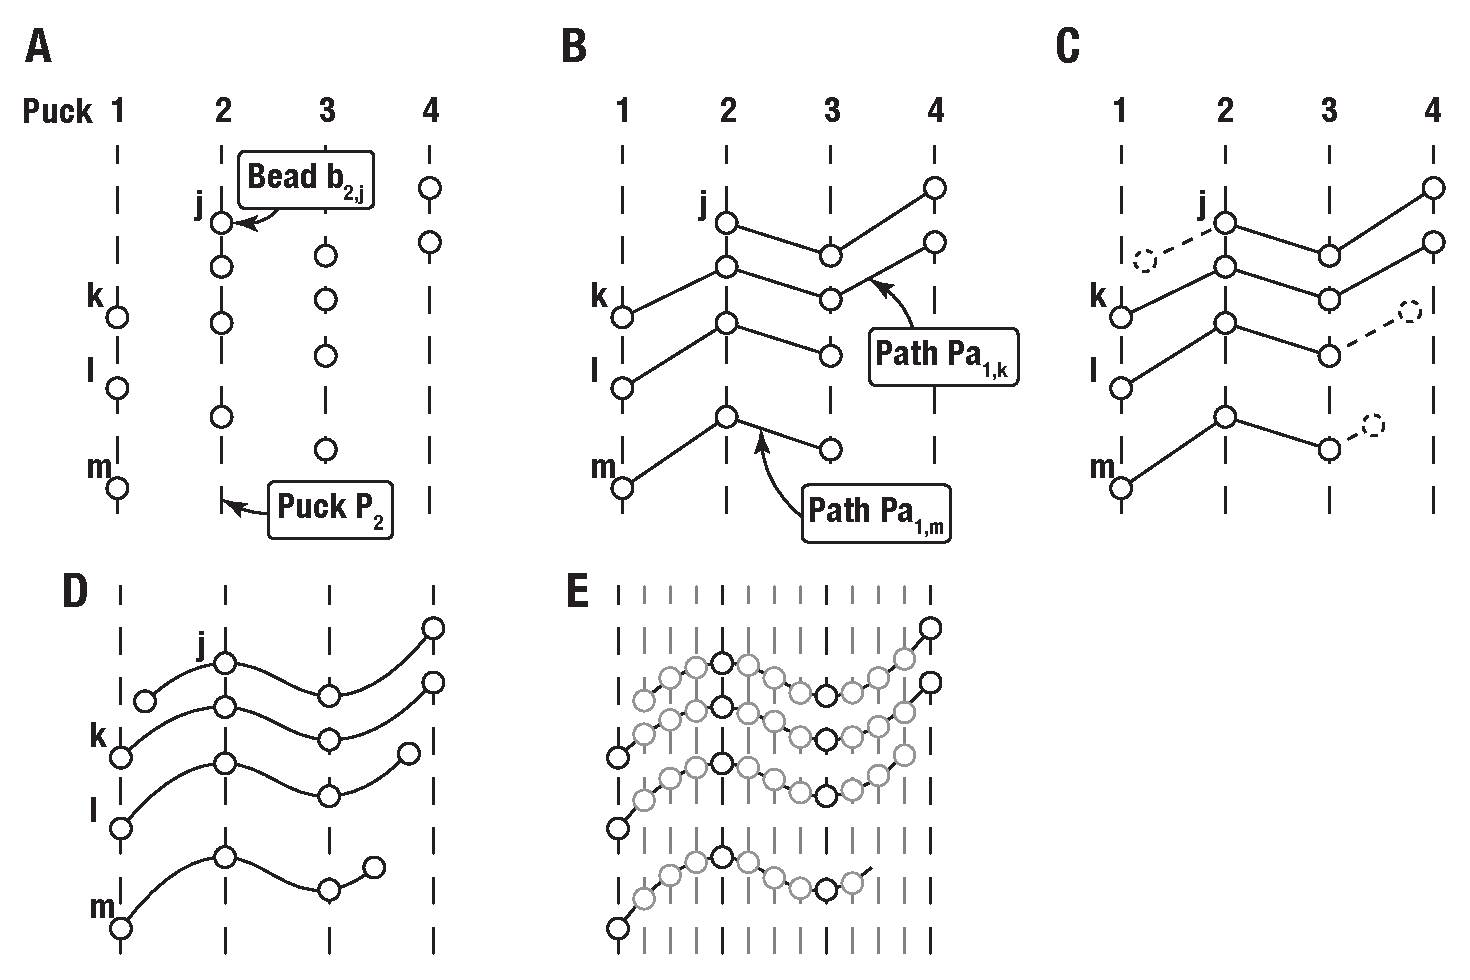
\includegraphics[width=0.8\textwidth]{figures/interpolation}
\caption{\textbf{Schematics of inter array bead interpolation.} A. Schematics of original data. Dashed lines represent the arrays, circles represent the beads. B. Pairing between beads of consecutive arrays forming the different paths. C. When necessary, addition of the in-between array projections. D. Resulting splines from the bead paring. E. Interpolation of beads in between the arrays, the grey beads are the interpolated ones.}\label{fig:interp}
\end{figure}
\subsection{Interpolation from the paths}
\paragraph{}Once the paths are created, all existing beads belong to a single path.
From these paths, positions and gene expressions can be interpolated.
Here, we interpolated the positions and gene expressions in between arrays as univariate cubic splines. Therefore, it is possible to retrieve the set of beads that live at any given \(z\) position together with the interpolated gene expression (see Fig. \ref{fig:interp} D-E).
\section{Spatial differential expression}
\paragraph{}The goal here was to score genes on whether they were locally expressed or not within a given tissue.
To do so, we quantified if the set of genes that are considered expressing are spatially positioned next to each other.
The metric we decided to use is based on the fact that the average degree of a graph (or network) is related to the average degree of that graph with randomly removed nodes.
If a graph \(G\) has a density of \(d(G)=k\), then if a fraction \(f\) of nodes are removed randomly, building the new graph \(G'\) , the density of \(G'\)  is \(d(G')\sim k(1-f)\).
But, if the nodes are not distributed randomly but are rather spatially localised, then the density of the new graph will be higher than the expected value: \(d(G')>k(1-f)\).

\paragraph{}Having the previous paragraph in mind, it means that the more a gene expression will be localised, the further away the density of the graph of expressing beads will be from the expected value of $k(1-f)$
\paragraph{}In the context of our study, \(G = (V, E)\) is the graph where the vertices are the beads with their spatial positions.
Then, to build the set of edges \(E\) between the vertices we computed the Gabriel graph on \(V\).
Finally, the fraction of removed nodes (\(f\)) is the fraction of the total number of beads in which beads are not expressing a given gene.
\paragraph{}To compute \(f\) we first computed the expression threshold above which a bead is considered expressing.
The threshold was computed independently for each gene-tissue pair as the value that splits the distribution of expression values for each gene within each tissue into two classes (expressing and not expressing beads).
For that we used the Otsu method \citep{Otsu:1979} which splits a distribution into two classes such that the intra-class variance is minimum (and therefore maximising the inter-class variance).
For each gene \(g\), we therefore have computed a threshold \(O_{th}(g)\).
\paragraph{}Having split the beads in two separate classes, we create the new graph \(G'_{g} = (V'_g, E'_g)\) where \(V'_g=\{v\in V~|~O_{th}(g)<ge(g, v)\}\) with \(ge(g,v)\) is the expression of the gene \(g\) of the vertice (or bead) \(v\).
The set of edges \(E'_g\) is then the set of edges included in \(E_g\) such that both vertices of the edges in \(E'_g\) are in the set of expressing beads (\(V'_g\)): \(E'_g=\{(v_1, v_2) \in E_g~|~(v_1, v_2)\in {V'}_g^{2}\}\).
\(G'_g\) is the graph of connections between beads expressing a given gene \(g\).
\paragraph{}We then computed the densities of \(G_g\) and \(G'_g\) as followed:
\begin{equation}
d(G_g)=\frac{2.|E_g|}{|V_g|(|V_g|-1)}.
\end{equation}
The fraction of removed nodes is computed as \(f_g=1-\frac{|V'_g|}{|V_g|}\).
This value can be seen as the ratio of volume expressing a given gene over the total volume.
We also normalised the values so they are comparable across different genes and tissues, we are therefore looking at \(f_g\) (which is already normalised) and \(d_g=\frac{d(G'_g)}{d(G_g)}\).
\paragraph{}We can then look at \(d_g\) against \(f_g\) knowing that \(d(G'_g)\sim d(G_g)f_g\) and therefore \(d_g\sim f_g\).
Because of the potential noise of the dataset, instead of taking the theoretical value, we computed the linear regression between the distributions \(d_g\) and \(f_g\) for each gene within a given tissue.
Then, for each gene, the distance to the linear regression is calculated which is the score for spatially expressed genes.
The higher the score, the further the gene is from the expected value, and therefore the further it is from being randomly expressed in space, meaning that it is locally expressed.

\section{Comparison to PASTE}
\paragraph{}We compared the results of our inter-array registration algorithm to the ones of PASTE described in \cite{Zeira:2022}.
The main difference between sc3D registration method and PASTE's is that our method relies heavily on the pre-annotation of the tissues of the dataset.
PASTE on the other hand only uses RNAI counts per bead and finds the transformation that minimises the difference between paired beads across arrays.
For that reason PASTE allows to perform array registration without having to pre-process the data as much as sc3D but sc3D is usually significantly faster since the optimisation part is done at a higher level.
\paragraph{}To compare PASTE to sc3D we used both our dataset and the human dorsolateral prefrontal cortex (DLPFC) from \cite{Maynard:2021} that was used in the PASTE article.
When we ran PASTE on the DLPFC dataset we used the optimal parameters provided by the article.
When we ran PASTE on our dataset, we tried different parameterisation and kept the best.
To compare our results to those of PASTE we used a similar metric than the one used in the PASTE article for non simulated datasets: the fraction of beads that have their closest bead in the neighbouring arrays belonging to the same tissue.
To compute our accuracy metric, we first compute a pairing between beads of consecutive arrays.
The pairing is a spatial proximity pairing where two beads are paired if they are closed spatially.
Effectively we computed the optimal pairing \(\pi^\star\) over the set of all the possible pairings \(\Pi\) that minimises the sum of the distances between paired beads:
\begin{equation}
\pi^\star = \argmin_{\pi\in \Pi}\sum_{(b_{i,j}, b_{i+1,k})\in \pi} \left\Vert b_{i,j}, b_{i+1,k}\right\Vert_2
\end{equation}
where \((b_{i,j}, b_{i+1,k})\in \pi\) are two paired beads in \(\pi\). To do so we used the Hungarian algorithm that gives an optimal result.
Given this pairing, we can now count the percentage of pairs that have the same tissue over the total number of pairs. The higher this percentage is, the better the alignment.
Figures \ref{fig:qual-DLPFC} and \ref{fig:qual-Mouse} show the accuracy of the alignment between our method and PASTE.
Note that for the DLPFC the results are similar and that for the mouse dataset sc3D performs better.
It is important to keep in mind that the parameterization that we found for PASTE on our dataset might not be the best even though we tried to optimise it.
\begin{figure}
\center
\includegraphics[width=0.8\textwidth]{figures/sc3D_vs_PASTE_DLPFC}
\caption{\textbf{Quality of alignment for PASTE and sc3D methods for the DLPFC dataset.}}\label{fig:qual-DLPFC}
\end{figure}
\begin{figure}
\center
\includegraphics[width=0.8\textwidth]{figures/sc3D_vs_PASTE_Mouse}
\caption{\textbf{Quality of alignment for PASTE and sc3D methods for our Mouse dataset at E8.5.} The subset of tissues for the second histogram is the following: Allantois, PP ectoderm, LPM, Somites, Heart, Brain, PSM, NMPs, Neural crest, Pharyngeal arch, Neural tube}\label{fig:qual-Mouse}
\end{figure}
\paragraph{}As another point of comparison, we recorded the time it took the two methods to align multiple arrays. We found our method to be one to two orders of magnitude faster (Figure \ref{fig:time-mouse}) on our dataset.
\begin{figure}
\center
\includegraphics[width=0.8\textwidth]{figures/sc3D_vs_PASTE_time}
\caption{\textbf{Processing time for the Mouse dataset}}\label{fig:time-mouse}
\end{figure}
\bibliographystyle{apalike}
\bibliography{references}
\end{document}